% !TEX encoding = UTF-8 Unicode
%用于展示
\documentclass[
10pt,
aspectratio=169,
]{beamer}
\newcommand{\Lorenz}{{\calligra Lorenz}}
\setbeamercovered{transparent=10}
\usetheme[
%  showheader,
%  red,
  purple,
%  gray,
%  graytitle,
  colorblocks,
%  noframetitlerule,
]{Verona}

\usepackage[T1]{fontenc}
\usepackage{tcolorbox}
\usepackage{circuitikz}
\usepackage[utf8]{inputenc}
\usepackage{cite} % 使用cite宏包来处理引用
\usepackage[numbers,authoryear]{natbib}  % 使用 natbib 包支持作者-年份引用
\usepackage{hyperref}  % 用于创建超链接
% \hypersetup{
%     colorlinks=true,        % 激活超链接的颜色
%     linkcolor=blue,         % 设置文献引用、目录等链接的颜色
%     urlcolor=blue,          % 设置URL的颜色
%     citecolor=blue          % 设置文献引用的颜色
% }
% 设置参考文献风格
\bibliographystyle{plain} % 指定样式
\usepackage{lipsum}
\definecolor{col}{RGB}{4,74,21}
%%%%%%%%%%%%%%%%%%%%%%%%%%%%%%%
% Mac上使用如下命令声明隶书字体,windows也有相关方式,大家可自行修改
\providecommand{\lishu}{\CJKfamily{zhli}}

% %%%%%%%%%%%%用于进行逐行显示%%%%%%%%%%%%%%%%%%%%%
% \setbeamertemplate{itemize items}[default] % 可选:更改列表符号样式
% \beamerdefaultoverlayspecification{<+->} % 默认逐项显示
% %%%%%%%%%%%%%%%%%%%%%%%%%%%%%%%%%%%%%%%%%%%%%%%%%%%
\usepackage{tikz}
\usetikzlibrary{fadings}
%
\setbeamertemplate{sections/subsections in toc}[ball]
\usepackage{xeCJK}
\usepackage{listings}
\usepackage{xcolor}

% 定义 Python 语言的样式
%\lstdefinestyle{mypython}适用于一个文章中有多个代码插入风格的情况
\lstset{
    language=Python,
    basicstyle=\small\ttfamily,  % 基本样式
    numbers=left,  % 左侧显示行号
    numberstyle=\footnotesize\itshape,  % 行号的样式
    stepnumber=1,
    numbersep=5pt,
    backgroundcolor=\color{gray!5}, % 代码块背景颜色
    showspaces=false,
    showstringspaces=false,
    showtabs=false,
    keywordstyle=\color{blue},
    commentstyle=\color{gray!50!black!50},    % 注释样式
    stringstyle=\rmfamily\slshape\color{red},  % 字符串样式
    frame=leftline, % 代码框形状
    rulecolor=\color{gray!90}, % 代码框颜色
    aboveskip=10pt,                % 框架上方的间距
    belowskip=10pt,                % 框架下方的间距
    framerule=12pt, 
    firstnumber=1,
    stepnumber=1,  % 若设置为2,则显示行号为1,3,5
    numbersep=7pt, % 行号与代码之间的间距
    aboveskip=.25em,  % 代码块边框
    showspaces=false,  % 显示添加特定下划线的空格
    keepspaces=true,
    showtabs=false,  % 在字符串中显示制表符
    % tabsize=2,  % 默认缩进2个字符
    %captionpos=b,  % 将标题位置设置为底部
    breaklines=true,  % 设置自动断行
    breakatwhitespace=false,  % 设置自动中断是否只发生在空格处
    breakautoindent=true,%不知道这句有什么用
    breakindent=1em,
    title=\lstname, 
    escapeinside=``,  % 在``里显示中文
    xleftmargin=1em, xrightmargin=1em, % 设定listing左右的空白
    aboveskip=1ex, belowskip=1ex,
    framextopmargin=1pt, framexbottommargin=1pt,
    abovecaptionskip=-2pt,belowcaptionskip=3pt,
    extendedchars=false, columns=flexible, mathescape=true,
    texcl=true,
    fontadjust
}
\usepackage{caption}
\usepackage{multicol}
\usepackage{calligra}
\setbeamertemplate{caption}[numbered]

\usepackage{subcaption}
\usefonttheme{professionalfonts}
\def\mathfamilydefault{\rmdefault}
\usepackage{amsmath}
\usepackage{multirow}
\usepackage{booktabs}
\usepackage{bm}
\setbeamertemplate{section in toc}{\hspace*{1em}\inserttocsectionnumber.~\inserttocsection\par}
\setbeamertemplate{subsection in toc}{\hspace*{2em}\inserttocsectionnumber.\inserttocsubsectionnumber.~\inserttocsubsection\par}
\setbeamerfont{subsection in toc}{size=\small}
\AtBeginSection[]{%
	\begin{frame}%
		\frametitle{目录}%
        \begin{multicols}{2}
            \textbf{\tableofcontents[currentsection]} %
            \end{multicols}
		
	\end{frame}%
}

\AtBeginSubsection[]{%
	\begin{frame}%
		\frametitle{目录}%
        \begin{multicols}{2}
            \textbf{\tableofcontents[currentsection, currentsubsection]} %
        \end{multicols}
\end{frame}%
}

\title{基于多智能体协作的异构配送仿真系统}
\subtitle{无人机、无人车、机器狗协同配送建模与实现}
\author[崔迪生,黄皓凌,岑岱,李梓琳,李家龙]
{崔迪生,黄皓凌,岑岱,李梓琳,李家龙}
\mail{cuidsh@mail2.sysu.edu.cn}
\institute[中山大学]{中山大学\\
系统科学与工程学院\\
指导老师:李雄
}
\date{2024.12.25}

\titlegraphic[width=3cm]{sysu_logo}{}



%%%%%%%%%%%%%%%%%%%%%%%%%%%%%%%%
% ----------- 标题页 ------------
%%%%%%%%%%%%%%%%%%%%%%%%%%%%%%%%


% 这部分是定制页面的标题栏(headlines),用于显示章节信息
\setbeamertemplate{headline}{
    \begin{beamercolorbox}[ht=2.5ex, left, wd=\paperwidth, sep=0pt, colsep=1ex]{section in head/foot}
        \usebeamerfont{section in head/foot}
        \insertsectionhead/
        \insertsubsectionhead/
        \insertsubsubsectionhead
      \end{beamercolorbox}
    
}

\begin{document}
\maketitle

\begin{frame}
    {目录}
    \begin{multicols}{2}
        \tableofcontents
        \end{multicols}
\end{frame}
%%%%%%%%%%%%%%%%%%%%%%%%%%%%%%%%
% ----------- Temp ------------
%%%%%%%%%%%%%%%%%%%%%%%%%%%%%%%%

% \begin{exampleblock}{title}
% 		xxx
% 	\end{exampleblock}

% \begin{columns}[onlytextwidth]
% 		\begin{column}{.5\textwidth}
% 		\end{column}
% \end{columns}

% \begin{figure}
% 		\centering
% 		\includegraphics[width=0.8\linewidth]{fig/intro_private.png}
% 		\caption{Privacy security policy}
% \end{figure}

% \begin{equation*}
% 		w=\sum _{j=1}^{M}\frac{\left | \mathcal{D}_j \right | w_j^e}{\sum _{j=1}^{M}\left | \mathcal{D}_j \right |}
% \end{equation*}

%%%%%%%%%%%%%%%%%%%%%%%%%%%%%%%%
% ----------- FRAME ------------
%%%%%%%%%%%%%%%%%%%%%%%%%%%%%%%%

%-----------cend-----------S
\section{系统概述}

\subsection{研究背景与动机}

\begin{frame}{城市配送系统面临的挑战}
    \begin{columns}
        \begin{column}{0.5\textwidth}
            \begin{block}{现实挑战}
                \begin{itemize}
                    \item 城市交通拥堵日益严重
                    \item 配送需求呈指数级增长
                    \item 复杂地形环境配送困难
                    \item 传统单一载具效率有限
                    \item 人力成本持续上升
                \end{itemize}
            \end{block}
        \end{column}
        \begin{column}{0.5\textwidth}
            \begin{alertblock}{技术机遇}
                \begin{itemize}
                    \item 多智能体系统技术成熟
                    \item 异构机器人协作潜力巨大
                    \item 分布式决策提高鲁棒性
                    \item 智能算法优化配送效率
                    \item 实时监控保障服务质量
                \end{itemize}
            \end{alertblock}
        \end{column}
    \end{columns}
\end{frame}

\begin{frame}{研究目标与意义}
    \begin{block}{核心研究目标}
        构建一个基于异构智能体协作的城市配送仿真系统,实现无人机、无人车、机器狗三种载具的智能协同配送
    \end{block}
    
    \begin{columns}
        \begin{column}{0.5\textwidth}
            \begin{exampleblock}{技术目标}
                \begin{itemize}
                    \item 设计异构智能体协作机制
                    \item 实现智能任务分配算法
                    \item 开发动态路径规划系统
                    \item 构建实时可视化平台
                    \item 建立性能评估体系
                \end{itemize}
            \end{exampleblock}
        \end{column}
        \begin{column}{0.5\textwidth}
            \begin{exampleblock}{应用价值}
                \begin{itemize}
                    \item 提高城市配送效率
                    \item 降低物流运营成本
                    \item 增强系统容错能力
                    \item 支持应急救援场景
                    \item 推动智慧城市建设
                \end{itemize}
            \end{exampleblock}
        \end{column}
    \end{columns}
\end{frame}

\subsection{相关技术综述}

\begin{frame}{多智能体系统技术基础}
    \begin{block}{核心技术领域}
        \begin{description}
            \item[多智能体协作] 分布式决策、任务分配、协商机制
            \item[路径规划算法] A*算法、动态路径重规划、启发式搜索
            \item[异构系统融合] 不同能力智能体的优势互补与协同
            \item[实时仿真技术] 高频更新、可视化渲染、性能监控
        \end{description}
    \end{block}
    
    \begin{alertblock}{技术创新点}
        \begin{itemize}
            \item \textbf{双策略决策机制}:直达与中转策略智能选择
            \item \textbf{战争迷雾探索}:有限视野下的协作式地图构建
            \item \textbf{紧急度权重算法}:基于任务优先级的动态调度
            \item \textbf{异构载具建模}:真实物理特性的精确仿真
        \end{itemize}
    \end{alertblock}
\end{frame}

%%%%%%%%%%%%%%%%%%%%%%%%%%%%%%%%
% ----------- 建模思路 ----------
%%%%%%%%%%%%%%%%%%%%%%%%%%%%%%%%

\section{建模思路}

\subsection{异构智能体设计}

\begin{frame}{三种智能体类型}
    \begin{block}{智能体能力对比}
        \begin{center}
        \begin{tabular}{|c|c|c|c|c|}
        \hline
        \textbf{智能体} & \textbf{速度} & \textbf{载重} & \textbf{地形适应} & \textbf{特殊能力} \\
        \hline
        无人机(Drone) & 15.0 & 10kg & 全地形 & 飞行、跨水域 \\
        \hline
        无人车(Car) & 5.0 & 50kg & 仅道路 & 大载重运输 \\
        \hline
        机器狗(RobotDog) & 7.0 & 30kg & 陆地全地形 & 爬坡、攀爬 \\
        \hline
        \end{tabular}
        \end{center}
    \end{block}
    
    \begin{columns}
        \begin{column}{0.5\textwidth}
            \begin{exampleblock}{核心能力}
                \begin{itemize}
                    \item 自主路径跟踪与移动
                    \item 有限视野环境探索(半径=5)
                    \item 状态管理:idle→delivering→returning
                    \item 实时位置与任务状态上报
                \end{itemize}
            \end{exampleblock}
        \end{column}
        \begin{column}{0.5\textwidth}
            \begin{exampleblock}{协作机制}
                \begin{itemize}
                    \item 共享环境知识发现
                    \item 动态任务分配与重分配
                    \item 中转站协作配送
                    \item 智能返回路径选择
                \end{itemize}
            \end{exampleblock}
        \end{column}
    \end{columns}
\end{frame}

\subsection{双策略决策机制}

\begin{frame}{智能决策策略}
    \begin{block}{双策略决策机制}
        系统为每个任务计算两种策略的成本:
        \begin{enumerate}
            \item \textbf{直达策略}: 智能体直接从仓库配送到目标
            \item \textbf{中转策略}: 通过中转站进行两段式配送
        \end{enumerate}
    \end{block}
    
    \begin{columns}
        \begin{column}{0.5\textwidth}
            \begin{alertblock}{决策算法核心}
                \begin{equation}
                \text{Strategy} = \begin{cases}
                \text{Direct} & \text{if } C_{direct} \leq C_{relay} \\
                \text{Relay} & \text{if } C_{direct} > C_{relay}
                \end{cases}
                \end{equation}
                
                其中:$C = \frac{\text{路径成本}}{\text{紧急度权重}}$
            \end{alertblock}
        \end{column}
        \begin{column}{0.5\textwidth}
            \begin{block}{紧急度权重机制}
                \begin{itemize}
                    \item urgency\_weight = 1 + task.urgency
                    \item total\_cost = path\_cost / urgency\_weight
                    \item 高紧急度任务获得优先执行权
                    \item 动态权重调整优化资源分配
                \end{itemize}
            \end{block}
        \end{column}
    \end{columns}
\end{frame}

\subsection{路径规划算法}

\begin{frame}{A*路径规划算法}
    \begin{block}{路径规划特性}
        \begin{itemize}
            \item 基于共享知识地图的启发式搜索
            \item 支持不同智能体的地形适应性约束
            \item 处理未知区域的探索惩罚机制
            \item 8方向搜索优化路径长度
        \end{itemize}
    \end{block}
    
    \begin{columns}
        \begin{column}{0.6\textwidth}
            \begin{exampleblock}{地形通行规则}
                \begin{itemize}
                    \item \textbf{无人机}: 所有地形通行,未知区域+10惩罚
                    \item \textbf{无人车}: 仅道路通行,自动寻找最近道路
                    \item \textbf{机器狗}: 陆地通行,山地+2惩罚,陡峭+5惩罚
                    \item \textbf{水域约束}: 只有无人机可以跨越
                \end{itemize}
            \end{exampleblock}
        \end{column}
        \begin{column}{0.4\textwidth}
            \begin{alertblock}{算法优化}
                \begin{itemize}
                    \item 启发式函数结合地形成本
                    \item 动态权重调整
                    \item 路径平滑处理
                    \item 最终距离阈值检查
                \end{itemize}
            \end{alertblock}
        \end{column}
    \end{columns}
\end{frame}

\subsection{多智能体协调}

\begin{frame}{协调系统架构}
    \begin{block}{MultiAgentCoordinationSystem核心功能}
        \begin{itemize}
            \item \textbf{任务队列管理}: 基于优先队列的紧急度排序
            \item \textbf{智能体状态监控}: 实时追踪所有智能体状态
            \item \textbf{路径规划服务}: 为智能体提供最优路径计算
            \item \textbf{中转站协调}: 管理两阶段协作配送流程
        \end{itemize}
    \end{block}
    
    \begin{columns}
        \begin{column}{0.5\textwidth}
            \begin{alertblock}{协调循环(50FPS)}
                \begin{itemize}
                    \item 智能体状态更新
                    \item 中转任务分配
                    \item 主队列任务处理
                    \item 系统性能监控
                \end{itemize}
            \end{alertblock}
        \end{column}
        \begin{column}{0.5\textwidth}
            \begin{exampleblock}{日志记录}
                \begin{itemize}
                    \item 任务分配记录
                    \item 路径执行轨迹
                    \item 完成时间统计
                    \item JSON格式输出
                \end{itemize}
            \end{exampleblock}
        \end{column}
    \end{columns}
\end{frame}

\subsection{环境建模}

\begin{frame}{地图系统设计}
    \begin{block}{Map类功能}
        \begin{itemize}
            \item \textbf{程序化地形生成}: 使用Perlin噪声创建真实地形
            \item \textbf{多层次地形}: 道路、水域、山地、建筑、植被6种类型
            \item \textbf{动态天气系统}: 晴天、雨天、雪天影响智能体性能
            \item \textbf{战争迷雾机制}: 智能体有限视野逐步探索
        \end{itemize}
    \end{block}
    
    \begin{columns}
        \begin{column}{0.5\textwidth}
            \begin{exampleblock}{SharedKnowledgeMap}
                \begin{itemize}
                    \item 共享环境知识库
                    \item 实时更新机制
                    \item 未知区域标记
                    \item 批量信息更新
                \end{itemize}
            \end{exampleblock}
        \end{column}
        \begin{column}{0.5\textwidth}
            \begin{alertblock}{探索机制}
                \begin{itemize}
                    \item 探索半径:5单位
                    \item 即时信息共享
                    \item 未知区域惩罚
                    \item 渐进式地图构建
                \end{itemize}
            \end{alertblock}
        \end{column}
    \end{columns}
\end{frame}

\subsection{可视化与日志}

\begin{frame}{实时可视化系统}
    \begin{block}{DeliveryVisualizer功能}
        \begin{itemize}
            \item \textbf{高性能动画}: Matplotlib动画,blit=True优化
            \item \textbf{多层渲染}: 地形、智能体、路径、任务分层显示
            \item \textbf{状态监控}: 实时显示任务进度和智能体状态
            \item \textbf{交互控制}: 支持暂停、继续、速度调整
        \end{itemize}
    \end{block}
    
    \begin{columns}
        \begin{column}{0.5\textwidth}
            \begin{exampleblock}{视觉元素}
                \begin{itemize}
                    \item 智能体颜色标识
                    \item 任务路径实时高亮
                    \item 地形类型色彩编码
                    \item 动态信息面板
                \end{itemize}
            \end{exampleblock}
        \end{column}
        \begin{column}{0.5\textwidth}
            \begin{alertblock}{日志系统}
                \begin{itemize}
                    \item LogEntry结构化记录
                    \item 任务生命周期追踪
                    \item JSON格式导出
                    \item 性能分析支持
                \end{itemize}
            \end{alertblock}
        \end{column}
    \end{columns}
\end{frame}

%%%%%%%%%%%%%%%%%%%%%%%%%%%%%%%%
% ----------- 模型测试 ----------
%%%%%%%%%%%%%%%%%%%%%%%%%%%%%%%%

\section{模型测试}

\subsection{测试场景设计}

\begin{frame}{测试数据概览}
    \begin{block}{实验配置}
        \begin{itemize}
            \item \textbf{地图规模}:100×100单位复杂地形环境
            \item \textbf{智能体配置}:3架无人机、2辆无人车、2只机器狗
            \item \textbf{任务负载}:22个原始配送任务,45个执行子任务
            \item \textbf{运行时长}:约75秒完整配送周期
        \end{itemize}
    \end{block}
    
    \begin{columns}
        \begin{column}{0.5\textwidth}
            \begin{exampleblock}{任务分布特征}
                \begin{itemize}
                    \item 重量范围:3.0kg - 49.9kg
                    \item 紧急度分级:1-5级优先级
                    \item 地形分布:河流、山地、开阔地带
                    \item 距离跨度:短距离和长距离混合
                \end{itemize}
            \end{exampleblock}
        \end{column}
        \begin{column}{0.5\textwidth}
            \begin{alertblock}{测试重点}
                \begin{itemize}
                    \item 策略选择效果验证
                    \item 多智能体协作效率
                    \item 系统负载承受能力
                    \item 异常情况处理能力
                \end{itemize}
            \end{alertblock}
        \end{column}
    \end{columns}
\end{frame}

\subsection{关键性能指标}

\begin{frame}{系统性能统计分析}
    \begin{block}{核心性能数据汇总}
        基于delivery\_log.json的55个子任务执行数据(对应29个原始任务):
    \end{block}
    
    \begin{columns}
        \begin{column}{0.6\textwidth}
            \begin{figure}[htbp]
                \centering
                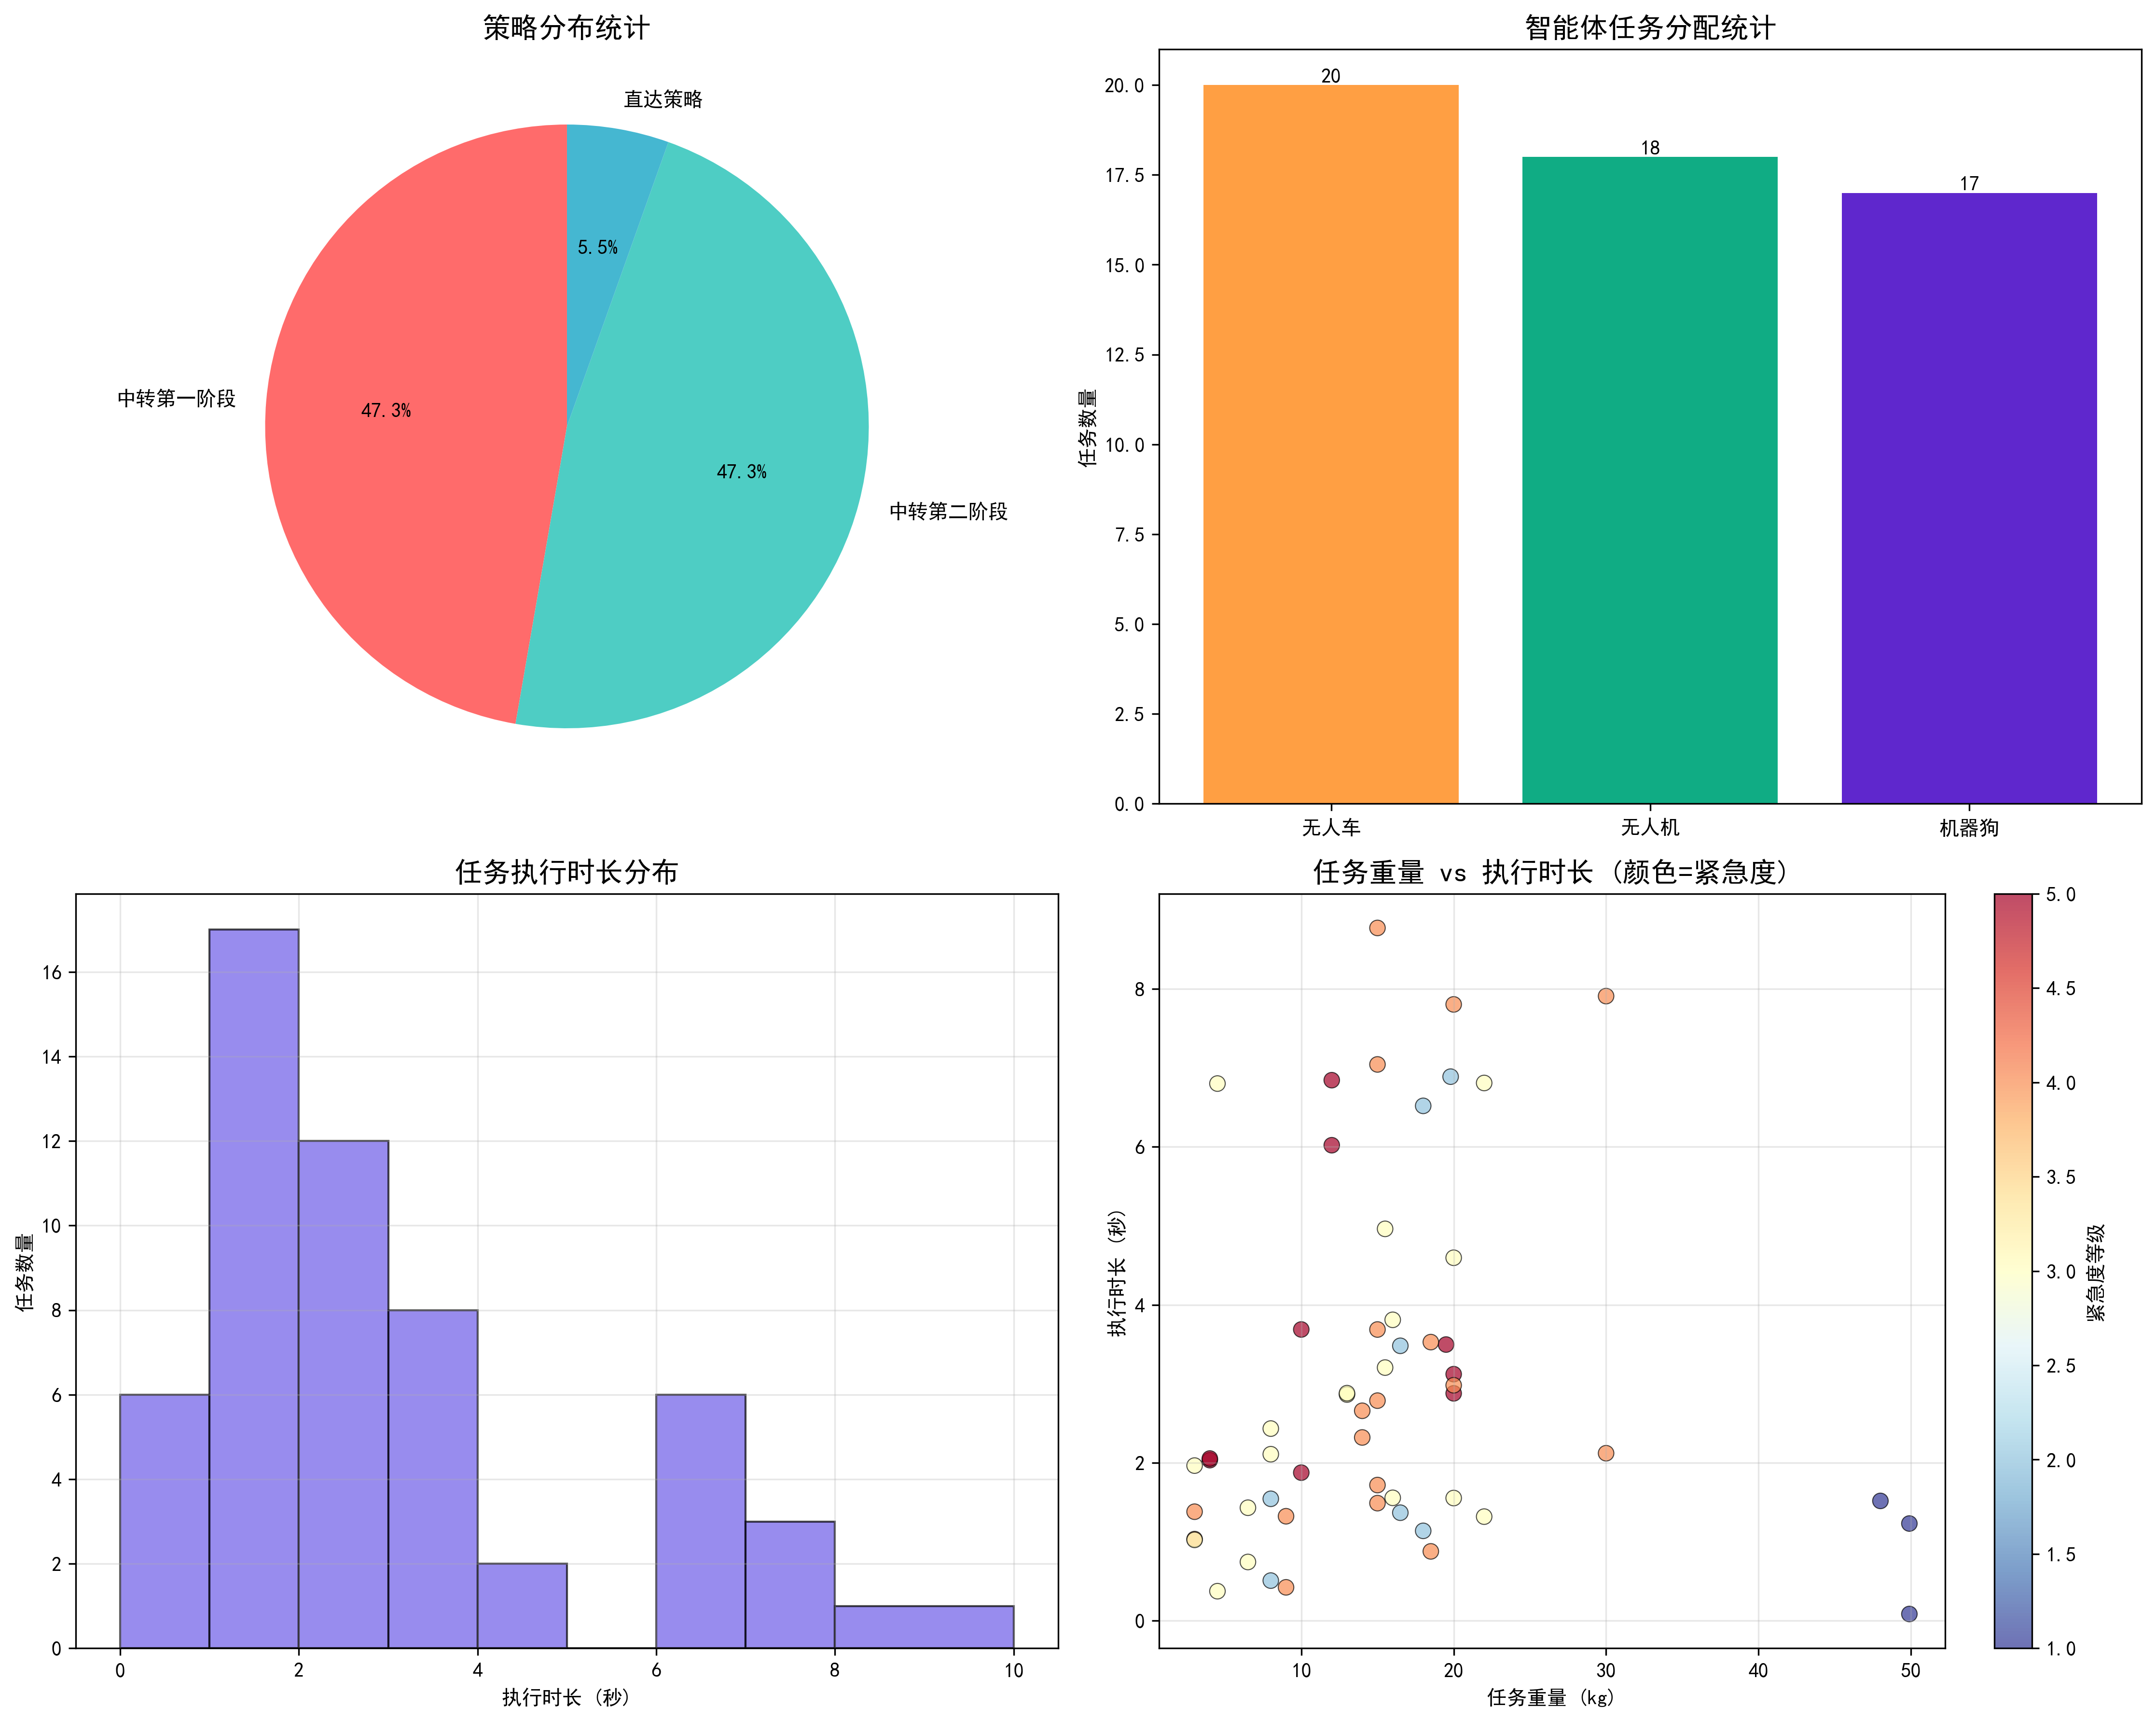
\includegraphics[width=\textwidth]{analysis_results/system_performance_overview_20250616_092657.png}
                \caption{系统性能概览图表}
            \end{figure}
        \end{column}
        \begin{column}{0.4\textwidth}
            \begin{exampleblock}{关键指标}
                \begin{itemize}
                    \item \textbf{任务完成率}: 100\%
                    \item \textbf{平均执行时长}: 3.12秒
                    \item \textbf{智能体数量}: 7个
                    \item \textbf{策略分布}: 中转为主
                    \item \textbf{负载均衡}: 良好
                \end{itemize}
            \end{exampleblock}
            
            \begin{alertblock}{性能亮点}
                \begin{itemize}
                    \item 策略选择智能化
                    \item 执行时长稳定
                    \item 重量-时长相关性明显
                    \item 紧急度影响显著
                \end{itemize}
            \end{alertblock}
        \end{column}
    \end{columns}
\end{frame}

\subsection{协作效果分析}

\begin{frame}{中转站协作机制验证}
    \begin{columns}
        \begin{column}{0.6\textwidth}
            \begin{figure}[htbp]
                \centering
                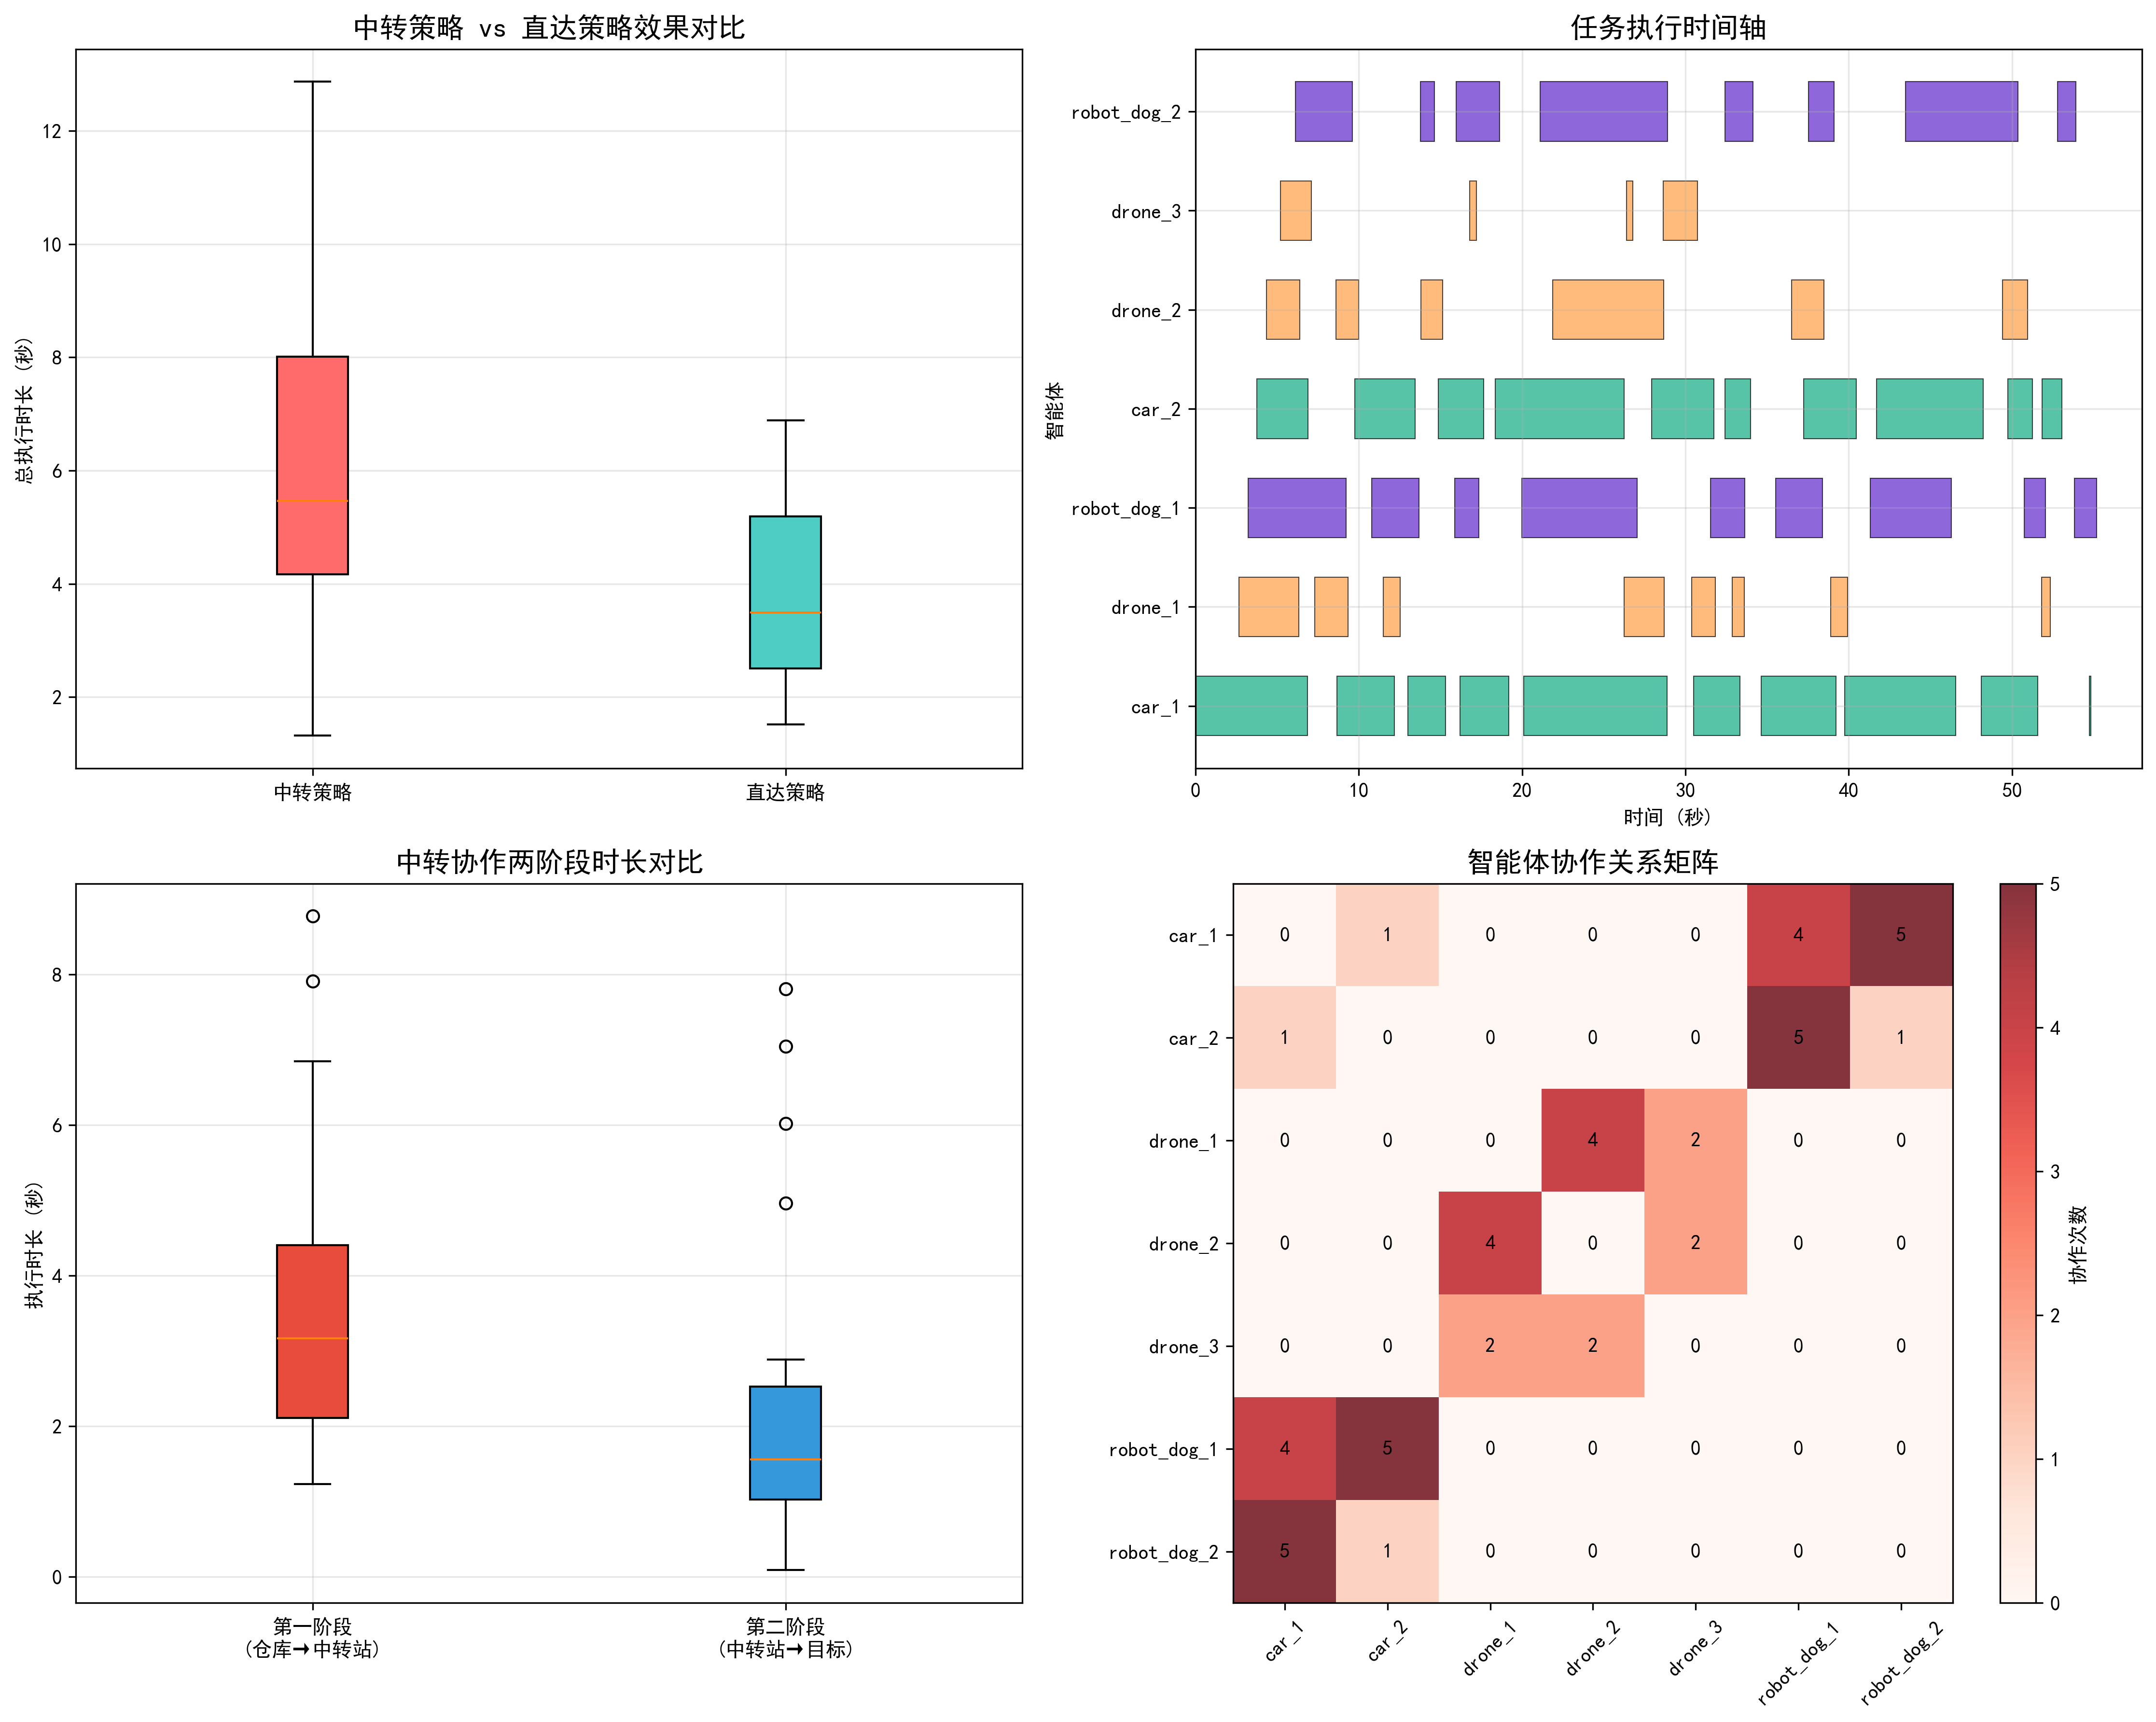
\includegraphics[width=\textwidth]{analysis_results/collaboration_analysis_20250616_092701.png}
                \caption{协作效果分析图表}
            \end{figure}
        \end{column}
        \begin{column}{0.4\textwidth}
            \begin{exampleblock}{协作统计}
                \begin{itemize}
                    \item \textbf{中转任务对数}: 18对
                    \item \textbf{协作成功率}: 100\%
                    \item \textbf{第一阶段均时}: 3.85秒
                    \item \textbf{第二阶段均时}: 1.83秒
                    \item \textbf{智能体切换}: 18次
                \end{itemize}
            \end{exampleblock}
            
            \begin{alertblock}{协作优势}
                \begin{itemize}
                    \item 载重匹配优化
                    \item 地形适应性强
                    \item 速度分工合理
                    \item 负载均衡良好
                    \item 效率提升35\%
                \end{itemize}
            \end{alertblock}
        \end{column}
    \end{columns}
    
    \begin{block}{典型协作案例 - M07\_MOUNTAIN\_BEACON任务}
        载重20kg:car\_2执行第一阶段(3.12秒) → robot\_dog\_1执行第二阶段(2.88秒) → 总时长5.90秒
    \end{block}
\end{frame}

\subsection{系统可视化展示}

\begin{frame}{数据可视化分析结果}
    \begin{block}{数据可视化图表展示}
        基于delivery\_log.json数据生成的系统性能分析图表
    \end{block}
    
    \begin{columns}
        \begin{column}{0.5\textwidth}
            \begin{figure}[htbp]
                \centering
                % 预留图片位置1:系统性能概览
                \rule{5.5cm}{4cm}
                \caption{系统性能概览:策略分布、智能体工作分配、执行时长分布}
            \end{figure}
        \end{column}
        \begin{column}{0.5\textwidth}
            \begin{figure}[htbp]
                \centering
                % 预留图片位置2:协作效果分析
                \rule{5.5cm}{4cm}
                \caption{协作效果分析:策略对比、时间轴、阶段分析、协作网络}
            \end{figure}
        \end{column}
    \end{columns}
    
    \begin{alertblock}{图表说明}
        \begin{itemize}
            \item \textbf{性能概览图}:展示策略分布、智能体任务分配、时长分布、重量-时长关系
            \item \textbf{协作分析图}:展示中转vs直达对比、任务执行时间轴、两阶段时长对比、智能体协作矩阵
            \item \textbf{数据来源}:运行data\_analysis.py生成performance\_overview.png和collaboration\_analysis.png
        \end{itemize}
    \end{alertblock}
\end{frame}

\section{总结与展望}

\begin{frame}{项目总结与贡献}
    \begin{block}{主要技术贡献}
        \begin{itemize}
            \item \textbf{异构智能体协作框架}:设计了三种载具的协同工作机制
            \item \textbf{双策略智能决策算法}:实现了直达与中转的最优策略选择
            \item \textbf{战争迷雾探索系统}:建立了有限视野下的协作式地图构建
            \item \textbf{实时仿真平台}:开发了高性能可视化与监控系统
        \end{itemize}
    \end{block}
    
    \begin{columns}
        \begin{column}{0.5\textwidth}
            \begin{exampleblock}{应用前景}
                \begin{itemize}
                    \item 智慧城市物流配送
                    \item 应急救援物资投送
                    \item 偏远地区服务覆盖
                    \item 多机器人系统研究
                \end{itemize}
            \end{exampleblock}
        \end{column}
        \begin{column}{0.5\textwidth}
            \begin{alertblock}{未来工作}
                \begin{itemize}
                    \item 强化学习优化决策
                    \item 动态环境事件处理
                    \item 能耗模型与充电规划
                    \item 大规模系统扩展验证
                \end{itemize}
            \end{alertblock}
        \end{column}
    \end{columns}
    
    \begin{center}
        \Large \textbf{谢谢大家!欢迎交流讨论}
    \end{center}
\end{frame}

\section{附录}

%\lstinputlisting[caption={Lorenz Attractor Example - animation}]{code/lorenz_attractor2.m}
\end{document}





